\documentclass[tikz,border=4pt]{standalone}
\usepackage{tikz}
\usetikzlibrary{shapes,arrows,positioning}
\begin{document}
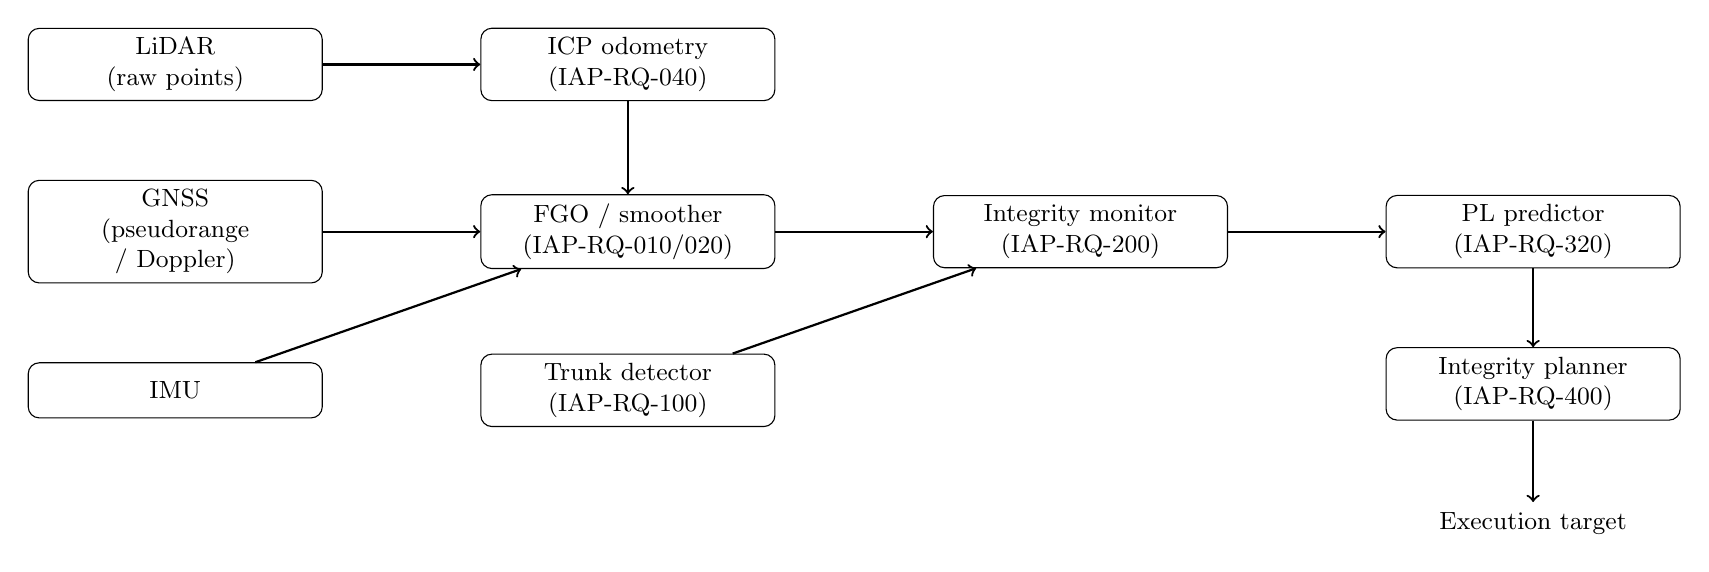
\begin{tikzpicture}[
    node distance=1.0cm and 1.6cm,
    block/.style={rectangle, draw, rounded corners, text width=3.5cm,
                  align=center, minimum height=0.7cm, font=\small},
    arrow/.style={->, thick}
  ]
  % ---- Sensing column ----
  \node[block] (lidar)  {LiDAR\\(raw points)};
  \node[block, below=of lidar] (gnss) {GNSS\\(pseudorange / Doppler)};
  \node[block, below=of gnss]  (imu)  {IMU};

  % ---- Processing ----
  \node[block, right=2.0cm of lidar]  (icp)  {ICP odometry\\(IAP-RQ-040)};
  \node[block, right=2.0cm of gnss]   (fgo)  {FGO / smoother\\(IAP-RQ-010/020)};
  \node[block, right=2.0cm of imu]    (trunk){Trunk detector\\(IAP-RQ-100)};

  % ---- Integrity ----
  \node[block, right=2.0cm of fgo]    (integ){Integrity monitor\\(IAP-RQ-200)};

  % ---- Planning ----
  \node[block, right=2.0cm of integ]  (pred) {PL predictor\\(IAP-RQ-320)};
  \node[block, below=of pred]         (plan) {Integrity planner\\(IAP-RQ-400)};

  % ---- Arrows ----
  \draw[arrow] (lidar) -- (icp);
  \draw[arrow] (gnss)  -- (fgo);
  \draw[arrow] (imu)   -- (fgo);
  \draw[arrow] (icp)   -- (fgo);
  \draw[arrow] (trunk) -- (integ);
  \draw[arrow] (fgo)   -- (integ);
  \draw[arrow] (integ) -- (pred);
  \draw[arrow] (pred)  -- (plan);
  \draw[arrow] (plan)  -- ++(0,-1.5) node[below, font=\small]{Execution target};
\end{tikzpicture}
\end{document}
